\documentclass{article}
\usepackage[utf8]{luainputenc}
\usepackage[T1]{fontenc}
\usepackage[a4paper,margin=0.75in, bottom=1in]{geometry}
\usepackage{listings}
\usepackage{minted}
\usepackage{courier}
\usepackage{amsmath}
\usepackage{amssymb}
\usepackage{enumerate}
\usepackage{graphicx}
\usepackage{hyperref}

\begin{document}
	
	\hrulefill
	\begin{center}
		\bfseries % Fettdruck einschalten
		\sffamily % Serifenlose Schrift
		\begin{huge}
			GTI: Grundlagen der Theoretischen Informatik
		\end{huge}\\
		\begin{Large}
			Sommersemester 2017, 2. Übungsblatt
		\end{Large}\\
		\begin{small}
			Christopher Husemann, Luis Herrmann; Tutor: Kristin Knorr; Mo 12:00-14:00
		\end{small}
		
		\vspace{-10pt}
	\end{center}
	\hrulefill
	
\section*{Aufgabe 1 - \textit{Einelementiges Alphabet}}
\begin{enumerate}[a)]
	\item Wir betrachten die Sprache $L = \{1^z | z = 3m + 5n \land m,n\in \mathbb{N}\}$. Die Sprache enthält die Unärdarstellungen von 0,3,5,6,8,9,10,11,12,... usw. Man kann sich leicht überzeugen, dass alle natürlich Zahlen $\ge 8$ als Zahl $z = 3m + 5n$, mit $m,n \in \mathbb{N}$ gebildet werden können. Beweis in 3 Schritten:
	\begin{enumerate}[1.]
		\item Alle $z \ge 8$ mit  $(z \mod 3) = 0$ sind in $L$:
		
		Sei $z \mod 3 = 0 \Rightarrow \exists m \in \mathbb{N} : 3m= z \Rightarrow \exists m,n \in\mathbb{N}: z = 3m + 5n$ für $n = 0$.
		
		\item Alle $z \ge 8$ mit $(z \mod 3 ) = 1$ sind in $L$:
		
		Sei $z \mod 3 = 1 \Rightarrow \exists m \in\mathbb{N} : 3m + 1 = z$. Falls $ z \ge 10$ folgt $\exists m \ge 3: 3(m-3) + 10 = z \Rightarrow \exists \tilde{m},n \in \mathbb{N}: z = 3\tilde{m} + 5n$ für $n = 2$.
		
		\item Alle $z \ge 8$ mit $(z \mod 3 ) = 2$ sind in $L$:
		
		Sei $z \mod 3 = 2 \Rightarrow \exists m \in\mathbb{N}: 3m +2 = z$. Falls $ z \ge 8$ folgt $\exists m \ge 2 : 3(m-1) + 5 = z \Rightarrow \exists\tilde{m},n \in \mathbb{N}: 3\tilde{m} + 5n = z$ für $n = 1$.
	\end{enumerate}
	Damit ist die Aussage gezeigt. Für alle kleineren Unärdarstellungen, die akzeptiert werden, überlegt man sich schnell passende Wertepaare $(m,n)$: $0 \to (0,0)$, $3 \to (1,0)$, $5 \to (0,1)$, $6 \to (2,0)$.
	
	Die Umsetzung einer dfa ist entsprechend einfach:
	
	\begin{minipage}{\textwidth}
		\centering 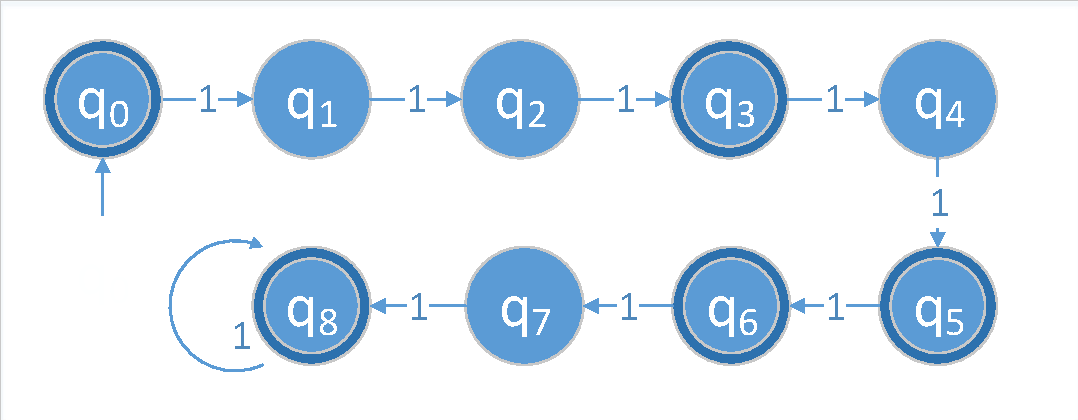
\includegraphics[width=0.8\textwidth,page=1,trim={2 2 2 4},clip]{dfas.pdf}
	\end{minipage}
	
	\item Da es in dfa's über einem einstelligen Alphabet zu einem gegebenen Zustand immer genau einen Nachfolgezustand gibt halten wir zunächst fest, dass wir die Zustände gemäß der Reihenfolge ihrer Ausführung für ein Wort maximaler Länge durchnummerieren können, also haben wir Zustände $Q = \{q_0,q_1, ..., q_n\}$. Es kann höchstens eine Schleife auftreten, denn angenommen es gibt ein Wort $w = u1v$ mit $|u| = i$, sodass $q_i$ ein Zustand der Automaten $A_L$ für Eingabe $w$ ist - also $\delta^*(q_0,u) = q_i$ - und es gilt zum ersten Mal $\delta(q_i,w) = q_j$ mit $j \le i$, dann gilt wegen $j \le i$ für $|v| = j -i$ auch $\delta^*(q_i,1v) = q_i$.
	
	Ferner folgt, dass $q_i$ der letzte Zustand in der Nummerierung ist, sodass unsere Schleife, sofern vorhanden, von $q_n$ geschlossen werden soll. Sei $q_j$ nun jener Zustand, sodass $\delta(q_n,1) = q_j$ mit $j \le n$. Dann existiert eine Menge von akzeptierenden Zuständen $q_i$ in $\{q_0, ..., q_{j-1}\}$ und $q_k$ in $\{q_j, ..., q_n\}$, die wir durch Indexmengen $I$ und $K$ charakterisieren können. Formal:
	\begin{equation}
		I := \{q \in \{q_0,...,q_{j-1}\} | q \in F\}, \quad K := \{q \in \{q_j,...,q_n\} | q \in F\}
	\end{equation}
	
	\begin{minipage}{\textwidth}
		\centering\includegraphics[width=\textwidth,page=2,trim={2 2 2 4},clip]{dfas.pdf}
	\end{minipage}
	
	Dann ist klar, dass wir den regulären Ausdruck $\alpha$, der die Sprache $L$ charakterisiert, wie folgt schreiben können:
	\begin{equation}
		\alpha = \bigvee\limits_{i\in I} 1^i \lor \bigvee\limits_{k \in K}1^k \left(1^{n-k+1}\right)^*
	\end{equation}
	
	Dabei steht der mit Kleene-Stern versehene Ausdruck bei der Veroderung über $K$ für die beliebig vielen, (n-k+1) Schritte langen Schleifendurchläufe, die man in $A_L$ unternehmen kann, ehe man wieder auf den akzeptierenden Zustand $q_k$ zurückkehrt.
	
\end{enumerate}

\section*{Aufgabe 2 - \textit{Zustandsdiagramm nfa}}

\begin{enumerate}[a)]
	\item Sei $N = (Q, \Sigma, s_0, \delta, F)$ ein nfa, dann ist der äquivalente dfa gegeben durch $A = (\mathcal{P}(Q), \Sigma, E(s_0), \delta', F')$ mit $\delta'(R,a) ) \{q \in Q | q\in E(\delta(r,a)) für ein r\in R \}$ und $F = \{R \in \mathcal{P}(Q) | R\cap F \neq \emptyset\}$. Wir erhalten somit folgende dfa:
	
	\begin{minipage}{\textwidth}
		\centering\includegraphics[width=\textwidth,page=3,trim={2 2 2 4},clip]{dfas.pdf}
	\end{minipage}
	
	\item Auf den nächsten Zettel verschoben.
\end{enumerate}

\section*{Aufgabe 3 - \textit{nfa versus dfa}}

	\begin{minipage}{\textwidth}
		\centering\includegraphics[width=0.8\textwidth,page=4,trim={2 2 2 4},clip]{dfas.pdf}
	\end{minipage}\\
	
	Durch den Loop in $q_0$ kann die Überprüfung für jedes eingelesene Zeichen neu gestartet werden.
	
\section*{Aufgabe 4 - \textit{nfa ohne $\epsilon$-Übergänge}}

Wir wählen einen nfa $N_\epsilon$ mit $\epsilon$-Übergängen $N_\epsilon = (Q,\Sigma,q_0,\delta_\epsilon,F_\epsilon)$ und konstruieren daraus den nfa $N_{\setminus\epsilon}$ ohne $\epsilon$-Übergänge $N_{\setminus\epsilon} = (Q,\Sigma,q_0,\delta_{\setminus\epsilon},F_{\setminus\epsilon})$. Dabei definieren wir die Übergangsfunktion wie folgt:

\begin{equation}
	\delta_{\setminus\epsilon}(q,a) = \begin{cases}
		q, &a = \epsilon\\
		\bigcup_{p \in E(q)}\delta_\epsilon(p,a), &a \in \Sigma
	\end{cases}
\end{equation}

wobei $E(q)$ der $\epsilon$-Abschluss von dem entsprechenden $q$ ist; somit ist $q \in E(q)$ und alle von $q$ in 0 Schritten erreichbaren Zustände, wobei:
\begin{equation}
	F_{\setminus\epsilon} = \begin{cases}
	F_\epsilon \cup \{q_0\}, &\text{wenn aus } E(q_0) \text{ ein } q \in F_\epsilon   \\ F_\epsilon, &\text{sonst}
	\end{cases}
\end{equation}

\section*{Aufgabe 5 - \textit{Abschlusseigenschaften}}
\begin{enumerate}[a)]
	\item Da wir in der Vorlesung gezeigt haben, dass die Regularität einer formalen Sprache äquivalent zu der Existenz eines dfa ist, welcher genau alle Wörter der Sprache akzeptiert, setzen wir für Sprachen $L_1$, $L_2$ deren Regularität vorausgesetzt wird, die Existenz eines dfa voraus. Schließlich zeigen wir, dass sich ein dfa konstruieren lässt, der die gewünschte Sprache akzeptiert, womit wir gezeigt haben, dass die gewünschte Sprache ebenfalls regulär ist.
	
	Wir definieren die dfa's wie folgt: $A(L_1) = (Q_1,\Sigma, q_{1,0}, \delta_1, F_1)$ $A(L_2) = (Q_2,\Sigma, q_{2,0}, \delta_2, F_2)$.
	
	(i) z.Z.  $L_3 = L_1 \cap L_2 \implies L_3$ ist reguläre Sprache.
	
	Wir konstruieren den dfa $A(L_3) := (Q, \Sigma, q_0, \delta, F)$ mit:
	\begin{align}
		Q := Q_1 \times Q_2,\quad 
		q_0 = (q_1,q_2), \quad
		\delta((q_1,q_2),a) = (\delta_1(q_1,a),\delta(q_2,a)),\quad 
		F = F_1 \times F_2
	\end{align}
	
	Die zugrundeliegende Idee ist, die Berechnenung von $A(L_1)$ und $A(L_2)$ parallel auf einem Eingabewort $w \in \Sigma^*$ durchzuführen. Offenbar ist $w \in L_1 \cap L_2$ gdw. $A(L_1)$ und $A(L_2)$ das Wort $w$ akzeptieren, dass heißt die Berechnung von $w$ endet in beiden Automaten auf einem akzeptieren Zustand. Die Menge aller $w \in L_1 \cap L_2$ ist in $A(L_3)$ also die Menge $\{ (q_1,q_2) \in Q_1\times Q_2 | q_1 \in F_1 \land q_2 \in F_2 \} = F_1 \times F_2$.
	
	(ii) z.Z $L_1^c = \Sigma^* \setminus L_1$ ist reguläre sprache.
	
	Macht man bei enem dfa $A(L_1)$ aus all seinen akzeptierenden Zutsänden nich-akzeptierende und aus nicht-akzeptierenden akzeptierende, so erhält man den dfa zu komplementären Sprache $L_1^c$, da dieser ein Wort $w$ genau dann akzeptiert (also $w \in L^c$), wenn der Automat $A(L_1)$ es nicht akzeptiert, also wenn $w \in L$.
	
	Man erhält den dfa zur komplementären, regulären Sprache also wie folgt:
	\begin{equation}
		L_1^c= (Q_1, \Sigma, q_{1,0}, \delta_1, Q_1 \setminus F_1 )
	\end{equation}
	
	(iii) z.Z  $L_3 = L_1 \setminus L_2$ ist reguläre Sprache.
	
	Da $L_1 \setminus L_2 = L_1 \cup L_2^c$ ist $L_3$ nach (i) und (ii) regulär.
	
	\item Sei $A(L_1)$ ein dfa, der für ein Wort $x$ der Länge $n+1$ entscheidet, ob $x_1...x_nx_{n+1} \in L$. Dann muss $A(L_1)$ auch für $x_1 ... x_n$ entscheiden, ob sich das Wort in der Sprache befindet. Induktiv folgt, dass $L$ für beliebige Präfixe eines Wortes entscheidet, ob sie sich in der Sprache befinden. Ist ein Präfix $x_1...x_i \in L$, dann befindet sich der Automat bei der Überprüfung von $x$ nach den ersten $i$ Schritten in einem akzeptierenden Zustand.\\
	
	\textbf{Idee 1: Konstruktion durch Kopie:}
	
	Die Konstruktionsidee für unseren dfa ist folgende: Erstelle eine Kopie $A'$ vom Automaten $A(L)$, welcher keine akzeptierenden Zustände hat. Sobald wir in einem Zustand landen, der in $A(L)$ akzeptierend wäre, gehe über zu dem entsprechenden Nachfolgezustand in $Q$. Durch diese Konstruktion landet man zum Schluss nur bei einem akzeptierenden Zustand, wenn sowohl das ganze Wort, als auch der Präfix in der Sprache $L$ liegen.
	
	Sei also $A(L) = (Q, \Sigma, q_0, \delta, F)$ mit $Q = \{q_0,...,q_n\}$. Dann konstruieren wir $A' = (Q', \Sigma, q_{-1}', \delta', \{\},)$ mit $Q' = \{q_0',...,q_n'\} \cup q_{-1}'$ wobei $q_i'$ eine Kopie von $q_i \in Q$ ist und
	$\delta'(q_{-1},a) = \delta'(q_0',a) $, wobei $\forall_i  \delta'(q_i',a) = q_j' \land \delta(q_i,a) = q_k \implies j = k$.
	
	Schließlich definieren wir noch die Kopierfunktion $C: Q' \setminus \{q_{-1}'\} \to Q$, welche $C(q_i') = q_i$ leistet.
	
	
	Mit dieser Vorarbeit definieren wir nun die dfa $A_\Phi = (Q \cup Q', \Sigma, q_{-q}', \delta_\phi, F)$ mit:
	\begin{equation}
		\delta_\phi(q,a) =  \begin{cases}
		\delta'(q,a) , &q \in Q'  \land C(q) \not\in F \\ \delta(C(q),a) , &q \in Q' \land C(q) \in F \\ \delta(q,a) , &q \in Q
		\end{cases}
	\end{equation}
	
	Der vorgeschaltete Zustand $q_{-1}$ sorgt dabei dafür, dass Worter der Länge $1$ nicht auf einen akzeptierenden Zustand führen können, denn wir betrachten hier $\epsilon$ nicht als echten Präfix (sonst wäre jedes Wort aus $L$ auch in $\Phi(L)$).\\
	
	\textbf{Idee 2: Konstruktion über parallele Berechnung:}
	
	Die Konstruktionsidee ist, eine parallele Berechnung auf dem Eingabewort durchzuführen, wobei die zweite Berechnung auf einem akzeptierenden Zustand verharren muss, sobald das erste Mal ein solcher auftaucht. Dazu definieren wir die dfa $A_\Phi := (Q_\Phi, \Sigma, s_\Phi, \delta_\Phi, F_\Phi)$ mit:
	\begin{align}
		&Q_\Phi = Q \times (Q \cup \{q_\text{ende}\}),\quad s_\Phi = (q_0,q_0)\quad F_\Phi = F \times \{q_\text{ende}\}\\
		&\delta_\Phi((q_1,q_2),a) = \begin{cases}
		(\delta(q_1,a),\delta(q_2,a)), &q_2 \not\in F\\
		(\delta(q_1,a),q_\text{ende}), &q_2 \in F\setminus\{ q_0\} \cup\{q_\text{ende}\}
		\end{cases}
	\end{align}
	
	Die Definition sorgt dafür, dass nur Wörter akzeptiert werden, die bei der ersten Berechnung durch $A(L)$ zum Schluss bei einem akzeptierenden Zustand landen UND zusätzlich bei der zweiten Berechnung irgendwann in einem Zustand landen, der in $A(L)$ akzeptierend ist, welcher bei Lesen des nächsten Zeichens bis Ende der Berechnung auf den Auszeichnungszustand $q_\text{ende}$ überführt wird.
	
	Offenbar führen das leere Wort und Wörter der Länge 1 nicht zum Akzeptieren des Automaten, da sich die zweite Berechnung zu Beginn nie in $q_\text{ende}$ befindet und durch nie nach Einlesen des ersten Zeichens auf $q_\text{ende}$ überführt werden kann. Erreicht die Berechnung durch $A(L)$ erst bei Lesen des letzten Zeichens einen akzeptierenden Zustand in $F$, so befindet sich die parallele Berechnung noch nicht in $q_\text{ende}$. Es werden also nur echte Präfixe akzeptiert.\\
	
	
	Da wir einen dfa konstruieren können, der genau die Worte aus $\Phi(L)$ akzeptiert, ist $\Phi(L)$ reguläre Sprache und somit eine Abschlusseigenschaft.
\end{enumerate}

\section*{Aufgabe 6 - \textit{Verständnisfragen}}
\begin{enumerate}[a)]
	\item Jede Teilmenge einer regulären Sprache ist regulär. Das ist eine falsche Aussage. Sei $\Sigma$ ein Alphabet, dann ist offenbar $\Sigma^*$ eine reguläre Sprache. Wäre jedes $L \subset \Sigma^*$ eine reguläre Sprache, dann wäre jede formale Sprache eine reguläre Sprache, was offenbar nicht zutrifft. Beispielsweise ist $\{0^n 1^n | n \in \mathbb{N}\} \subset \{0,1\}^*$ eine formale Sprache, aber keine reguläre Sprache, da sie sich nicht durch endliche Vereinigungen, Konkatenationen und Kleene-Operatoren erzeugen lässt. 
	
	\item Die Aussage ist wahr, denn $\text{Suff}_k(L)$ enthält höchstens $N = 1 \textbf{(leeres Wort )} + 2^0 + ... + 2^k = 2^{k+1}$ Wörter. Also lässt sich $\text{Suff}_k(L)$ durch eine endliche Vereinigung von einelementigen Mengen erzeugen und ist somit reguläre Sprache.
	
	\item Seien alle Sprachen aus $C$ diskunkt, d.h. $\forall L_1, L_2 \in C: L_1 \cap L_2 \neq \emptyset$. Sei ferner $C$ eine abzählbar unendlich große Menge. Wäre die Aussage wahr, wäre auch hier wieder jede formale Sprache $L \subseteq \Sigma^*$ über einem Alphabet $\Sigma^*$ eine reguläre Sprache, denn $\Sigma^*$ hat abzählbar unendlich viele Wörter. Das heißt, $\Sigma^*$ und folglich jede Teilsprache $L$ ließe sich als abzählbare Vereinigung einer abzählbaren Menge von Sprachen erzeugen (die zum Beispiel jeweils genau ein Element aus der Sprache enthalten).
	
	Wie das in der Vorlesung besprochene Beispiel aus a) verdeutlicht, ist aber nicht jede formale Sprache auch eine reguläre Sprache.
	
\end{enumerate}
	
	
	
	
\end{document}